\chapter{Backstepping}
Este es un método para construir una \gls{flc} para una clase especial de sistemas.\\

\rmk{
	También se puede encontrar en la literatura el \textit{Forwarding}, pero no se aborda debido a que es, en general, un método más complicado.
}
\section{El caso más simple: Backstepping de integrador}
La idea básica del método conocido como \textbf{backstepping} se puede explicar, en su forma más simple, considerando el sistema con entrada escalar
\begin{equation}
	\begin{aligned}
		\dot{\eta} & = f(\eta) + g(\eta)\xi                                    \\
		\dot{\xi}  & = u, \quad \eta \in \mathbb{R}, \quad \xi \in \mathbb{R}.
	\end{aligned}
	\label{eq: backstepping_integrador}
\end{equation}
Nótese que este sistema se puede ver como una conexión en cascada, donde el maestro es un integrador y el esclavo es el sistema no lineal $\dot{\eta} = f(\eta) + g(\eta)\xi$. El objetivo de control es estabilizar el origen utilizando retroalimentación de los estados.\\

La idea de Backstepping es escencialmente recursiva, es decir, partimos de pensar en $\xi$ como una variable de control \textit{virtual} para el sistema $\dot{\eta} = f(\eta) + g(\eta)\xi$ y queremos diseñar una ley de control para $\xi$ que estabilice al origen asintóticamente, es decir, buscamos estabilizar al esclavo de la cascada. La idea básica descrita a bloques, como se puede apreciar en la Figura \ref{fig: backstepping_bloques}.\\

\begin{figure}[H]
	\centering
	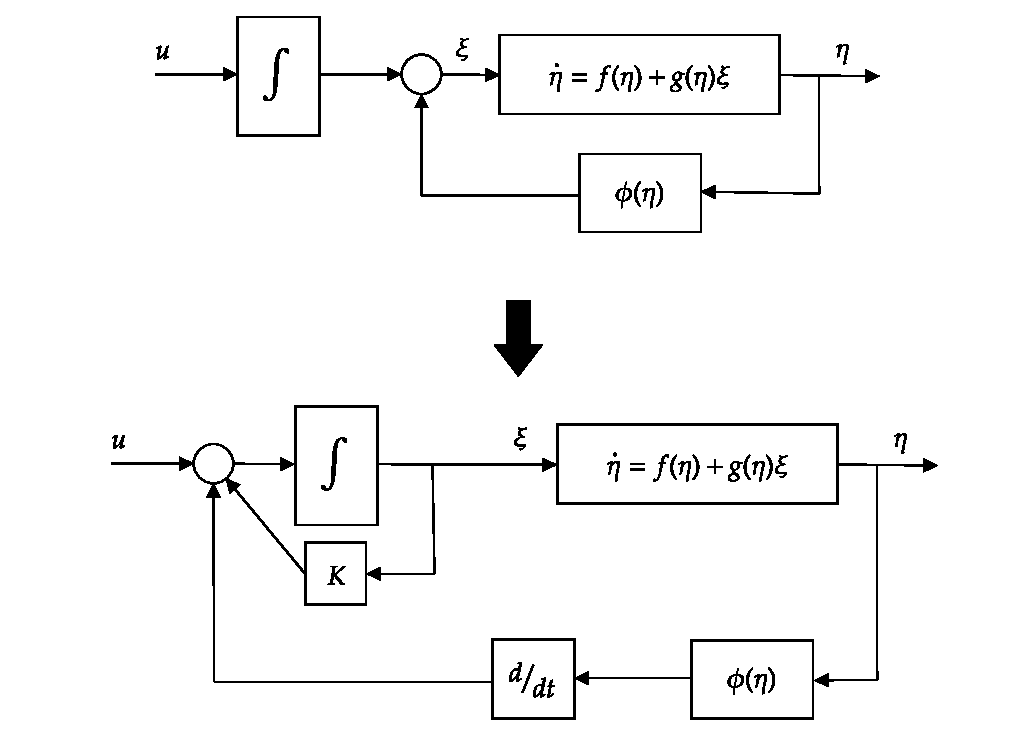
\includegraphics[width=0.8\textwidth]{img/backstepping_BlockDiagram.pdf}
	\caption{Idea básica del Backstepping de integrador.}
	\label{fig: backstepping_bloques}
\end{figure}

\subsection{Diseño del control virtual}
Véase a $\xi$ como una entrada de control virtual del sistema
\begin{equation}
	\dot{\eta} = f(\eta) + g(\eta)\xi.
	\label{eq: backstepping_esclavo}
\end{equation}
Suponga que existe una ley de control retroalimentado
\begin{equation*}
	\xi = \phi(\eta)
\end{equation*}
que estabiliza el origen de
\begin{equation*}
	\dot{\eta} = f(\eta) + g(\eta)\phi(\eta).
\end{equation*}
y que, además, conocemos una \gls{fl} $V(\eta)$ que lo asegura:

\begin{equation*}
	\dot{V}(\eta) = \dfrac{\partial(\eta)}{\partial \eta} [f(\eta) + g(\eta)\phi(\eta)] \leq -W(\eta), \quad \forall \eta \in D.
\end{equation*}

\subsection{Diseño del control verdadero por Backstepping}
\textbf{Cambio de coordenadas:} Como no se puede implementar el control virtual $\xi = \phi(\eta)$, definimos el error como una nueva variable
\begin{equation*}
	z = \xi - \phi(\eta).
\end{equation*}
Escribiendo el sistema en términos de esta nueva variable se obtiene
\begin{equation*}
	\begin{aligned}
		\dot{\eta} & = [f(\eta) + g(\eta)\phi(\eta)] + g(\eta)z,                                                         \\
		\dot{z}    & = u - \frac{\partial \phi(\eta)}{\partial \eta} [f(\eta) + g(\eta)\xi], \quad \xi = z + \phi(\eta).
	\end{aligned}
\end{equation*}
Si se diseña la variable de control como
\begin{equation*}
	u = -\dfrac{\partial \phi(\eta)}{\partial \eta} [f(\eta) + g(\eta)\xi] + v
\end{equation*}
entonces el sistema se describe como
\begin{equation}
	\begin{aligned}
		\dot{\eta} & = [f(\eta) + g(\eta)\phi(\eta)] + g(\eta)z, \\
		\dot{z}    & = v.
	\end{aligned}
	\label{eq: backstepping_z}
\end{equation}
\rmkb{
	¿Cuál es la diferencia entre \eqref{eq: backstepping_esclavo} y \eqref{eq: backstepping_z}? La diferencia es que en \eqref{eq: backstepping_z} el esclavo con la entrada proveniente del maestro igualada a cero $(z=0)$ tiene un \gls{pe} que es asintóticamente estable, esto es, el sistema es de Fase Mínima.\\

	En resumen, con un simple cambio de variables estabilizamos la \gls{dc} del sistema.\\

	Bastaría con estabilizar al maestro (que ya es lineal) y entonces el sistema completo tiene un \gls{pe} asintóticamente estable localmente (usando las ideas de linealización parcial).
}
La diferencia ahora, sin tomar el camino de Linealización Parcial, será construir una \gls{flc} para el sistema \eqref{eq: backstepping_z}, luego vamos a usar esa \gls{flc} para estabilizar al sistema completo \eqref{eq: backstepping_integrador}.

\subsubsection{Diseño del control por Lyapunov} El diseño se realiza proponiendo una \textbf{función candidata de Lyapunov}, en nuestro caso se puede usar
\begin{equation*}
	V_c(\eta, \xi) = V(\eta) + \dfrac{1}{2}z^2.
\end{equation*}
El control $v$ se elige de tal forma que $\dot{V}_c$:
\begin{equation*}
	\dot{V}_c = \underbrace{\dfrac{\partial V}{\partial \eta} [f(\eta) + g(\eta)\phi(\eta)]}_{<0} + \underbrace{\dfrac{\partial V(\eta)}{\partial \eta}g(\eta)z + zv}_{\text{diseñe } v}.
\end{equation*}
sea negativa definida. Aquí se propone
\begin{equation*}
	v = -\dfrac{\partial V(\eta)}{\partial \eta}g(\eta)z - kz, \quad k > 0.
\end{equation*}
con lo que
\begin{equation*}
	\dot{V}_c \leq -W(\eta) -kz^2,
\end{equation*}
donde
\begin{equation*}
	W(\eta) = \dfrac{\partial V(\eta)}{\partial \eta}g(\eta)z^2 - \dfrac{\partial V(\eta)}{\partial \eta}g(\eta)z.
\end{equation*}
El control $u$ finalmente, resulta ser
\begin{equation*}
	u = -\dfrac{\partial \phi(\eta)}{\partial \eta} [f(\eta) + g(\eta)\xi] - \dfrac{\partial V(\eta)}{\partial \eta}g(\eta)z - k(z + \phi(\eta)), \quad k > 0.
\end{equation*}
\rmkb{
	Note las siguientes diferencias importantes con respecto a la Linealización Parcial:
	\begin{itemize}
		\item La suma de las funciones de Lyapunov para los sistemas individuales se convierte en una función de Lyapunov para el sistema completo. Esto es gracias a la acción de control.

		\item El subsistema esclavo de la cascada no tiene que ser estable con entrada cero, sino que se puede estabilizar mediante el control virtual.
	\end{itemize}
}

\ex{
	Considere el sistema
	\begin{equation*}
		\begin{aligned}
			\dot{x}_1 &= x_1^2 - x_1^3 + x_2, \\
			\dot{x}_2 &= u, \quad \quad \quad  \quad \quad \quad x_1, x_2, u \in \mathbb{R}.
		\end{aligned}
	\end{equation*}
	Una ley de control virtual para el primer sistema
	\begin{equation*}
		x_2 = \phi(x_1) = - x_1 - x_1^2
	\end{equation*}
	estabiliza globalmente el origen de
	\begin{equation*}
		\dot{x}_1 = - x_1 - x_1^3
	\end{equation*}
	como lo prueba la función de Lyapunov
	\begin{equation*}
		V(x_1) = \dfrac{1}{2}x_1^2 \Rightarrow \dot{V}(x_1) = -x_1^2 - x_1^4 \leq 0, \quad \forall x_1 \in \mathbb{R}.
	\end{equation*}
	Introduciendo el siguiente cambio de variables
	\begin{equation*}
		z_2 = x_2 - \phi(x_1) = x_2 + x_1 + x_1^2
	\end{equation*}
	el sistema se puede reescribir como
	\begin{equation*}
		\begin{aligned}
			\dot{x}_1 &= - x_1 - x_1^3 + z_2, \\
			\dot{z}_2 &= u + (1+2x_1)(-x_1 - x_1^3 + z_2)
		\end{aligned}
	\end{equation*}
	Se propone como candidata de Lyapunov
	\begin{equation*}
		V_c(x) = \dfrac{1}{2}x_1^2 + \dfrac{1}{2}z_2^2
	\end{equation*}
	cuya derivada
	\begin{equation*}
		\begin{aligned}
			\dot{V}_c &= x_1(-x_1 - x_1^3 + z_2) + z_2[u + (1+2x_1)(-x_1 - x_1^3 + z_2)] \\
					  &= -x_1^2 - x_1^4 + z_2[x_1 + (1+2x_1)(-x_1 - x_1^3 + z_2) + u]
		\end{aligned}
	\end{equation*}
	y, eligiendo
	\begin{equation*}
		u = -x_1 - (1+2x_1)(-x_1 - x_1^3 + z_2) - z_2
	\end{equation*}
	hacemos a $\dot{V}_c$ negativa definida
	\begin{equation*}
		\begin{aligned}
			\dot{V}_c &= -x_1^2 - x_1^4 - z_2^2\\
					  &= -x_1^2 - x_1^4 - (x_2 + x_1 + x_1^2)^2
		\end{aligned}
	\end{equation*}
}

\ex{
	Considere el sistema
	Considere el sistema
	\begin{equation*}
		\begin{aligned}
			\dot{x}_1 &= x_1^2 - x_1^3 + x_2, \\
			\dot{x}_2 &= x_3, \\
			\dot{x}_3 &= u
		\end{aligned}
	\end{equation*}
	Para el sistema esclavo
	\begin{equation*}
		\begin{aligned}
			\dot{x}_1 &= x_1^2 - x_1^3 + x_2, \\
			\dot{x}_2 &= x_3
		\end{aligned}
	\end{equation*}
	una ley de control virtual es
	\begin{equation*}
		x_3 = -x_1 - (1+2x_1)(-x_1 - x_1^3 + x_2) - z_2 = \phi(x_1, x_2)
	\end{equation*}
	que estabiliza globalmente el origen, como lo prueba la función de Lyapunov
	\begin{equation*}
		V(x_1) = \dfrac{1}{2}x_1^2 + \dfrac{1}{2}x_2^2 \Rightarrow \dot{V} = -x_1^2 -x_1^4 - z_2^2 \leq 0, \quad \forall (x_1, x_2) \in \mathbb{R}^2.
	\end{equation*}
	Introduciendo el cambio de variables
	\begin{equation*}
		z_2 = x_3 - \phi(x_1, x_2)
	\end{equation*}
	el sistema se puede reescribir como
	\begin{equation*}
		\begin{aligned}
			\dot{x}_1 &= x_1^2 - x_1^3 + x_2 \\
			\dot{x}_2 &= \phi(x_1, x_2) + z_3 \\
			\dot{z}_3 &= u - \frac{\partial \phi}{\partial x_1}(x_1^2 - x_1^3 + x_2) - \frac{\partial \phi}{\partial x_2}(\phi + z_3)
		\end{aligned}
	\end{equation*}
	Se propone como candidata de Lyapunov
	\begin{equation*}
		V_c(x) = V(x_1, z_2) + \dfrac{1}{2}z_3^2
	\end{equation*}
	cuya derivada
	\begin{equation*}
		\begin{aligned}
			\dot{V}_c &= \dfrac{\partial V}{\partial x_1}(x_1^2 - x_1^3 + x_2) + \dfrac{\partial V}{\partial x_2}(\phi + z_3) \\
			&+ z_3\left[ u - \frac{\partial \phi}{\partial x_1}(x_1^2 - x_1^3 + x_2) - \frac{\partial \phi}{\partial x_2}(\phi + z_3)   \right] \\
			&= -x_1^2 - x_1^4 - (x_2 + x_1 + x_1^2)^2\\
			&+ z_3\left[ \frac{\partial V}{\partial x_2} - \frac{\partial \phi}{\partial x_1} (x_1^2 - x_1^3 + x_2) - \frac{\partial \phi}{\partial x_2} (z_3 + \phi) + u  \right]
		\end{aligned}
	\end{equation*}
	y eligiendo
	\begin{equation*}
		u = - \frac{\partial V}{\partial x_2} + \frac{\partial \phi}{\partial x_1} (x_1^2 - x_1^3 + x_2) + \frac{\partial \phi}{\partial x_2} (z_3 + \phi) - z_3
	\end{equation*}
	se hace negativa definida a $\dot{V}_c$.
}
\section{Un caso más general}
Un caso más general del método de Backstepping puede verse del sistema
\begin{equation}
	\begin{aligned}
		\dot{\eta} &= f(\eta) + g(\eta)\xi, \\
		\dot{\xi} &= f_a(\eta, \xi) + g_a(\eta, \xi)u, \quad g_a(\eta, \xi) \neq 0.
	\end{aligned}
	\label{eq: backstepping_general}
\end{equation}
donde $\eta \in \mathbb{R}^n$, $\xi, u \in \mathbb{R}$.\\

Mediante la ley de control
\begin{equation*}
	u = -\dfrac{1}{g_a(\eta, \xi)}\left[ v - f_a(\eta, \xi) \right]
\end{equation*}
el sistema se convierte en
\begin{equation}
	\begin{aligned}
		\dot{\eta} &= f(\eta) + g(\eta)\xi, \\
		\dot{\xi} &= v.
	\end{aligned}
	\label{eq: backstepping_general_v}
\end{equation}
\section{Forma de Retroalimentación Estricta}
Aplicando la idea anterior en forma recursiva, se puede concluir que la idea de Backstepping puede ser aplicada a sistemas en la forma de retroalimentación estricta, es decir, un sistema descrito por
\begin{equation*}
	\begin{aligned}
		\dot{x} &= f_0(x) + g_0(x)z_1, \\
		\dot{z}_1 &= f_1(x, z_1) + g_1(x, z_1)z_2, \\
		\dot{z}_2 &= f_2(x, z_1, z_2) + g_2(x, z_1, z_2)z_3, \\
		\vdots \\
		\dot{z}_{k-1} &= f_{k-1}(x, z_1, \ldots, z_{k-1}) + g_{k-1}(x, z_1, \ldots, z_{k-1})z_k, \\
		\dot{z}_k &= f_k(x, z_1, \ldots, z_k) + g_k(x, z_1, \ldots, z_k)u
	\end{aligned}
\end{equation*}
para todo $x \in \mathbb{R}^n$, $z_i \in \mathbb{R}$ y
\begin{equation*}
	g_i(x, z_1, \ldots, z_i) \neq 0, \quad \text{para } 1 \leq i \leq k.
\end{equation*}

\rmkb{
	Nótese que el subsistema $z$ es linealizable por retroalimentación. Así que el sistema en la forma de retroalimentación estricta es linealizable parcialmente (entarada/salida). Por lo que el Backstepping se aplica, escencialmente, a la clase de sistemas que son linealizables parcialmente.\\
}

\ex{
	Considere el sistema
	\begin{equation*}
		\begin{aligned}
			\dot{\eta} &= -\eta + \eta^2 \xi \\
			\dot{\xi} &= u .
		\end{aligned}
	\end{equation*}
	El sistema esclavo $\dot{\eta} = -\eta + \eta^2 \xi$, estabilizado con la ley de control virtual
	\begin{equation*}
		\xi = 0 \quad \Rightarrow \quad \dot{\eta} = -\eta
	\end{equation*}
	tiene un \gls{pe} \gls{gee}, y
	\begin{equation*}
		V_0 = \dfrac{1}{2}\eta^2 \Rightarrow \dot{V}_0 = -\eta^2, \quad \forall \eta \in \mathbb{R}.
	\end{equation*}
	es una \gls{fl}. Se propone como candidata a \gls{fl} a
	\begin{equation*}
		V = \dfrac{1}{2} (\eta^2 + \xi^2)
	\end{equation*}
	cuya derivada es
	\begin{equation*}
		\dot{V} = \eta(-\eta + \eta^2 \xi) + \xi u = -\eta^2 + \xi (\eta^3 + u),
	\end{equation*}
	que se puede hacer negativa definida eligiendo el control
	\begin{equation*}
		u = -\eta^3 - k\xi, \quad k > 0
	\end{equation*}
	\begin{equation*}
		\dot{V} = -\eta^2 - k\xi^2 < 0, \quad \forall (\eta, \xi) \in \mathbb{R}^2.
	\end{equation*}
}

\section{Backstepping en bloques}
La idea del backstepping puede generalizarse al sistema de múltiples entradas
\begin{equation*}
	\begin{aligned}
		\dot{\eta} = f(\eta) + G(\eta)\xi, \\
		\dot{\xi} = f_a(\eta, \xi) + G_a(\eta, \xi)u, \quad \det(G_a(\eta, \xi)) \neq 0.
	\end{aligned}
	\label{eq: backstepping_bloques}
\end{equation*}
donde $\eta \in \mathbb{R}^n$, $\xi \in \mathbb{R}^p$, $u \in \mathbb{R}^p$.\\

Suponga que existe una ley de control retroalimentado suave
\begin{equation*}
	\xi = \phi(\eta), \quad \phi(0) = 0
\end{equation*}
que estabiliza el origen de
\begin{equation*}
	\dot{\eta} = f(\eta) + G(\eta)\phi(\eta)
\end{equation*}
y que, además, conocemos una \gls{fl} $V(\eta)$, suave y positiva definida, que lo asegura
\begin{equation*}
	\dot{V}(\eta) = \dfrac{\partial V(\eta)}{\partial \eta} [f(\eta) + G(\eta)\phi(\eta)] \leq -W(\eta), \quad \forall \eta \in D,
\end{equation*}
para alguna función $W(\eta)$ positiva definida.\\

Considere la \gls{fl} candidata
\begin{equation*}
	V_c(\eta, \xi) = V(\eta) + \dfrac{1}{2}(\xi - \phi(\eta))^T(\xi - \phi(\eta)).
\end{equation*}
El control $u$ se elige de tal forma que $\dot{V}_c$:
\begin{equation*}
	\begin{aligned}
		\dot{V}_c &= \dfrac{\partial V(\eta)}{\partial \eta} [f(\eta) + G(\eta)\phi(\eta)] + \dfrac{\partial V(\eta)}{\partial \eta}G(\eta)(\xi - \phi(\eta)) \\
		&+ \left[\xi - \phi(\eta)\right]^T\left[ f_a(\eta, \xi) + G_a(\eta, \xi)u - \dfrac{\partial \phi(\eta)}{\partial \eta} (f(\eta) + G(\eta)\xi) \right] \\
	\end{aligned}
	\label{eq: backstepping_bloques_1}
\end{equation*}
sea negativa definida. El control
\begin{equation*}
	u = -G_a^{-1}(\eta, \xi)\left[ \dfrac{\partial \phi(\eta)}{\partial \eta} (f(\eta) + G(\eta)\xi) - \left(\dfrac{\partial V(\eta)}{\partial \eta}G(\eta)\right)^T - f_a(\eta, \xi) - k(\xi - \phi(\eta)) \right]
\end{equation*}
con $k>0$, resulta en
\begin{equation*}
	\begin{aligned}
		\dot{V}_c &= \dfrac{\partial V(\eta)}{\partial \eta} [f(\eta) + G(\eta)\phi(\eta)] - k(\xi - \phi(\eta))^T(\xi - \phi(\eta))
		&\leq -W(\eta) - k(\xi - \phi(\eta))^T(\xi - \phi(\eta))
	\end{aligned}
\end{equation*}
que muestra que el origen $(\eta, \xi) = (0, 0)$ es asintóticamente estable.\\

\section{Una versión (ligeramente) más general}
\subsection{Agregando un integrador}
Supóngase que se tiene un sistema que es equivalente por retroalimentación (transformación $+$ retroalimentación de estados) al sistema
\begin{equation*}
    \begin{aligned}
        \dot{x}_1 &= F(x_1, \textcolor{red}{x_2}), \quad \quad x_1 \in \mathbb{R}^{n-m}, \quad F(0,0) = 0 \\
        \dot{x}_2 &= u
    \end{aligned}
    \label{eq: backstepping_integrador_2}
\end{equation*}


